\subsubsection{Dézoomé}
L'opérateur dézoomé est l'opérateur le plus intéressant de Taggre, il permet d'effectuer des agrégations assez génériques et souvent efficaces.
%
En effet, cet opérateur va travailler à diminuer à la fois la largeur et la hauteur du graphe.
%
Abrégé {\em D} dans Taggre, cet opérateur essaye de créer des agrégats de tâches proche spatialement, un peu à la manière d'un partitionneur de graphe.
%
Le nom {\em dézoomé} provient du fait que la structure globale du graphe ne change pas beaucoup pendant l'agrégation même si le nombre de tâches a lui considérablement diminué.
%
Dans les meilleurs cas le nombre de tâches peut être divisé par le paramètre donné par le programmeur (Fig.~\ref{fig:algo_D4}).


L'algorithme \ref{algo:algo_D} permet d'implémenter l'opérateur dézoomé tout en assurant l'absence de création de cycle.
%
L'algorithme va simuler l'exécution des tâches et n'agrégera des tâches ensemble qui si le simulateur peut l'ordonnancer.
%
Les tâches ainsi agrégées sont ensuite simulées pour fournir de nouvelles tâches à agréger.



%   (-_-)   %
\begin{figure}[t!]
  \centering
  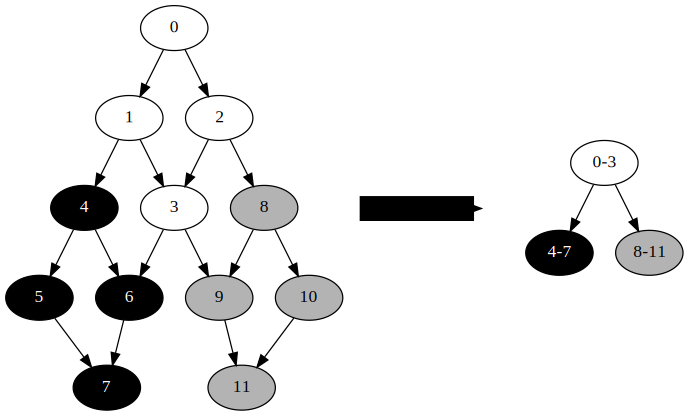
\includegraphics[width=0.8\textwidth]{algo_D4}
  \caption{Exemple d'utilisation de l'opérateur D avec le paramètre 4. Le nombre total de tâche a bien été divisé par 4.}
  \label{fig:algo_D4}
\end{figure}

\begin{algorithm}
  \KwData{DAG, $M$ : le nombre de tâches dans un agrégat}
  {\sc Prêt} = liste vide \\
  mettre les tâches racines de DAG dans {\sc Prêt} \\
  \While{{\sc Prêt} n'est pas vide} {
    {\sc Profondeur} = {\sc Prêt} \\
    {\sc Prêt} = liste vide \\
    \While{{\sc Profondeur} n'est pas vide} {
      {\sc Maître} = retirer le premier de {\sc Profondeur} \\
      {\sc Libérer} = liste vide \\
      mettre {\sc Maître} dans {\sc Libérer} \\
      {\sc Compteur} = 0 \\
      \While{{\sc Compteur} $< M$ {\bf et} {\sc Libérer} n'est pas vide} {
        {\sc Suivant} = retirer le premier de {\sc Libérer} \\
        {\sc Compteur}++\\
        agréger {\sc Maître} et {\sc Suivant}\\
        mettre les tâches libérées par {\sc Suivant} dans {\sc Libérer} \\
        trier {\sc Libérer} par nombre de précédence de {\sc Maître} \\
      }
      mettre les tâches libérées par {\sc Maître} dans {\sc Profondeur} \\
    }
    mettre les tâches libérées par {\sc Profondeur} dans {\sc Prêt}\\
  }
  \caption{Algorithme de l'opérateur dézoomé.}
  \label{algo:algo_D}
\end{algorithm}
